\chapter{Конструкторский раздел}
\label{cha:design}

В данном разделе будет приведено описание схем алгоритмов
сортировка пузырьком, сортировка вставками, сортировка слиянием
и вычислены их трудоемкости.

\section{Разработка алгоритмов}

На рисунках \ref{fig:2.1}, \ref{fig:2.2}, \ref{fig:2.3} показаны схемы алгоритмов сортировки.


% \pagebreak
\subsection{Сортировкa пузырьком}

\begin{figure}[h]
    \centering
    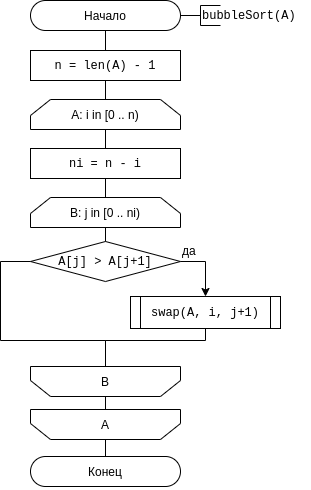
\includegraphics[width=0.48\textwidth]{3/inc/d1.png}
    \caption{Схема алгоритма сортировкa пузырьком}
    \label{fig:2.1}
\end{figure}


\newpage
\subsection{Сортировкa вставками}

\begin{figure}[h!]
    \centering
    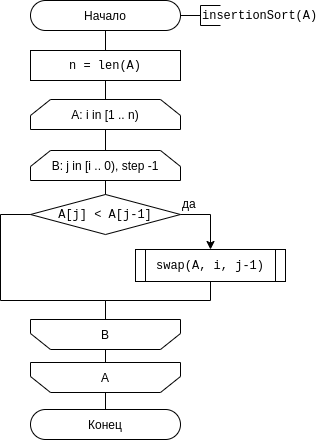
\includegraphics[width=0.52\textwidth]{3/inc/d2.png}
    \caption{Схема алгоритма сортировкa вставками}
    \label{fig:2.2}
\end{figure}

\newpage
\subsection{Сортировкa слиянием}

\begin{figure}[h!]
    \centering
    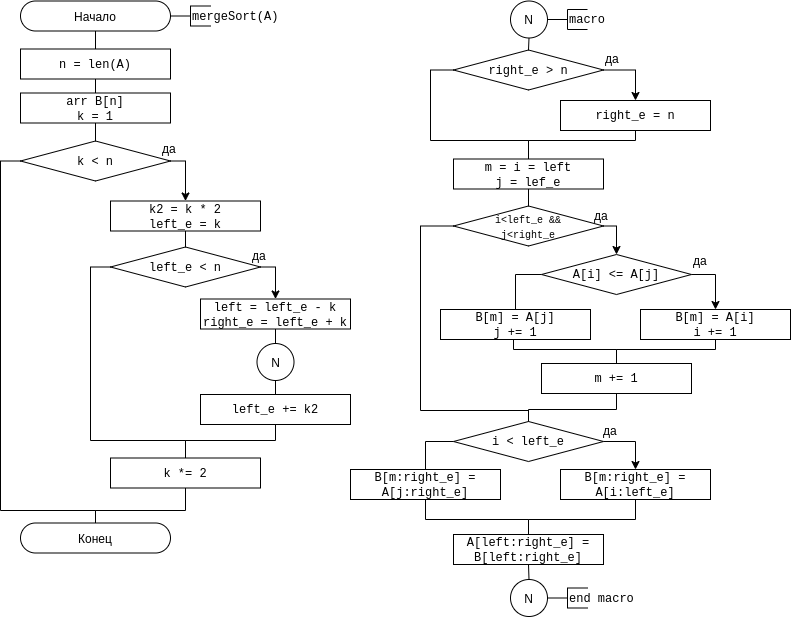
\includegraphics[width=1\textwidth]{3/inc/d3.png}
    \caption{Схема алгоритма сортировкa слиянием}
    \label{fig:2.3}
\end{figure}


\clearpage
\section{Оценка трудоемкости}

Применить формулы \ref{eq:1.1} и \ref{eq:1.2}.
Предположим, что сложность $swap()$ равна 5, сложность $len()$ равна n.

\subsection{Сортировкa пузырьком}


\begin{tabular}{|c|c|}
    \hline
    $F_{if}$        & $\left\{
        \begin{array}{ll}
            4, \hspace{0.5cm} $л.с.$\\
            9, \hspace{0.5cm} $х.с.$\\
        \end{array}
        \right.$ \\\hline\hline
    $F_{forA}$      & $\left\{
        \begin{array}{ll}
            4n + 6 \cdot \dfrac{(n-2)(n-1)}{2} = 3n^2 - 5n + 6, \hspace{0.5cm} $л.с.$\\
            4n + 11 \cdot \dfrac{(n-2)(n-1)}{2} = 5.5n^2 - 12.5n + 11, \hspace{0.5cm} $х.с.$\\
        \end{array}
        \right.$ \\\hline\hline
    $F_{bubble}$    & $\left\{
        \begin{array}{ll}
            3n^2 - 4n + 10, \hspace{0.5cm} $л.с.$\\
            5.5n^2 - 11.5n + 15, \hspace{0.5cm} $х.с.$\\
        \end{array}
        \right.$ \\\hline
\end{tabular}


\subsection{Сортировкa вставками}

\begin{tabular}{|c|c|}
    \hline
    $F_{if}$        & $\left\{
        \begin{array}{ll}
            4, \hspace{0.5cm} $л.с.$\\
            9, \hspace{0.5cm} $х.с.$\\
        \end{array}
        \right.$ \\\hline\hline
    $F_{forA}$      & $\left\{
        \begin{array}{ll}
            2n + 6 \cdot \dfrac{(n-2)(n-1)}{2} = 3n^2 - 7n + 6, \hspace{0.5cm} $л.с.$\\
            2n + 11 \cdot \dfrac{(n-2)(n-1)}{2} = 5.5n^2 - 14.5n + 11, \hspace{0.5cm} $х.с.$\\
        \end{array}
        \right.$ \\\hline\hline
    $F_{insert}$    & $\left\{
        \begin{array}{ll}
            3n^2 - 6n + 9, \hspace{0.5cm} $л.с.$\\
            5.5n^2 - 13.5n + 14, \hspace{0.5cm} $х.с.$\\
        \end{array}
        \right.$ \\\hline
\end{tabular}


\subsection{Сортировкa слиянием}

Алгоритм использует парадигма «разделяй и властвуй»,
делит массив на два меньших массива, сортирует его, а затем объединяет.
Шаг завоевания, на котором мы рекурсивно сортируем два подмассива примерно по n/2 элемента в каждом.
Шаг объединения объединяет в общей n элементов, что занимает время O(n).
В любом случае сложность сортировки слиянием $nlog_2n$.
(источник "Analysis of merge sort" \cite{b4}).


\section{Вывод}
В данном разделе было приведено описание схем алгоритмов и вычислены их трудоемкости.
